% Modelo de TCC do Bacharelado em Ciência da Computação da UNIFESP 
% Baseado no Modelo de Documentos Academicos do ABNTex2  

\documentclass[	12pt, Times, openright, oneside, a4paper, english, brazil]{abntex2}
% ---
% Pacotes fundamentais 
% ---
\usepackage{cmap}				% Mapear caracteres especiais no PDF
%\usepackage{lmodern}			% Usa a fonte Latin Modern			
\usepackage{times}
\usepackage[T1]{fontenc}			% Selecao de codigos de fonte.
\usepackage[utf8]{inputenc}		% Codificacao do documento (conversão automática dos acentos)
\usepackage{lastpage}			% Usado pela Ficha catalográfica
%\usepackage{natbib}
\usepackage{indentfirst}			% Indenta o primeiro parágrafo de cada seção.
\usepackage{color}				% Controle das cores
\usepackage{graphicx}			% Inclusão de gráficos
% ---

% ---
% Pacotes de citações
% ---
\usepackage[brazilian,hyperpageref]{backref}	 % Paginas com as citações na bibl
\usepackage[alf]{abntex2cite}	% Citações padrão ABNT

% --- 
% CONFIGURAÇÕES DE PACOTES
% --- 

% ---
% Configurações do pacote backref
% Usado sem a opção hyperpageref de backref
\renewcommand{\backrefpagesname}{Citado na(s) página(s):~}
% Texto padrão antes do número das páginas
\renewcommand{\backref}{}
% Define os textos da citação
\renewcommand*{\backrefalt}[4]{
	\ifcase #1 %
		Nenhuma citação no texto.%
	\or
		Citado na página #2.%
	\else
		Citado #1 vezes nas páginas #2.%
	\fi}%
% ---

% numeração de figuras e tabelas 
\counterwithout{figure}{section}
\counterwithout{table}{section}

%\renewcommand\tablename{Tabela{\arabic{chapter}.}}

% ---
% Informações de dados para CAPA e FOLHA DE ROSTO
% ---
\titulo{Modelos Explicativos com Inteligência Artificial Aplicados à Economia e Finanças}
\autor{Lucas de Oliveira Freitas}
\local{São José dos Campos, SP}
\data{Julho de 2025}
\orientador{Prof. Dr. Renato Cesar Sato}
% \coorientador{Prof. Dr. Beltrano da Silva}
\instituicao{%
  Universidade Federal de São Paulo -- UNIFESP
  \par
  Instituto de Ciência de Tecnologia
  \par
  Bacharelado em Ciência da Computação}
\tipotrabalho{Trabalho de Graduação}
% O preambulo deve conter o tipo do trabalho, o objetivo, 
% o nome da instituição e a área de concentração 
\preambulo{Trabalho de conclusão de curso apresentado ao Instituto de Ciência e Tecnologia – UNIFESP, como parte das atividades para obtenção do título de Bacharel em Ciência da Computação.}
% ---

% informações do PDF
\makeatletter
\hypersetup{
     	%pagebackref=true,
		pdftitle={\@title}, 
		pdfauthor={\@author},
    	pdfsubject={\imprimirpreambulo},
	    pdfcreator={LaTeX with abnTeX2},
		pdfkeywords={abnt}{latex}{abntex}{abntex2}{trabalho acadêmico}, 
		colorlinks=true,       		% false: boxed links; true: colored links
    	linkcolor=blue,          	% color of internal links
    	citecolor=blue,        		% color of links to bibliography
    	filecolor=magenta,      		% color of file links
		urlcolor=blue,
		bookmarksdepth=4
}

\makeatother
% --- 
% --- 
% Espaçamentos entre linhas e parágrafos 
% --- 
% O tamanho do parágrafo é dado por:
\setlength{\parindent}{1.3cm}
% Controle do espaçamento entre um parágrafo e outro:
\setlength{\parskip}{0.2cm}  % tente também \onelineskip
% ---

% compila o indice
% ---
\makeindex
% ---

% ----
% Início do documento
% ----
\begin{document}
% Retira espaço extra obsoleto entre as frases.
\frenchspacing 

% ----------------------------------------------------------
% ELEMENTOS PRÉ-TEXTUAIS
% ----------------------------------------------------------
% \pretextual

% ---
% Capa
% ---
\begin{capa}
  \begin{center}
   
\includegraphics[width=.25\textwidth]{logo-unifesp.pdf}
    \vspace*{\fill}
    
    {\ABNTEXchapterfont\large\imprimirautor}
    \vspace*{\fill}
    
    {\ABNTEXchapterfont\bfseries\Large\imprimirtitulo}
    \vspace*{\fill}\vspace*{\fill}
    
   \imprimirlocal
   \end{center}
\end{capa}

% ---
% Folha de rosto
% (o * indica que haverá a ficha bibliográfica)
% ---
\imprimirfolhaderosto*
% ---

% ---
% Inserir folha de aprovação
% ---
% Isto é um exemplo de Folha de aprovação, elemento obrigatório da NBR
% 14724/2011 (seção 4.2.1.3). Você pode utilizar este modelo até a aprovação
% do trabalho. Após isso, substitua todo o conteúdo deste arquivo por uma
% imagem da página assinada pela banca com o comando abaixo:
%
% \includepdf{folhadeaprovacao_final.pdf}
%
% \begin{folhadeaprovacao}
%   \begin{center}
%     {\ABNTEXchapterfont\large\imprimirautor}

%     \vspace*{\fill}\vspace*{\fill}
%     {\ABNTEXchapterfont\bfseries\Large\imprimirtitulo}
%     \vspace*{\fill}
    
%     \hspace{.45\textwidth}
%     \begin{minipage}{.5\textwidth}
%         \imprimirpreambulo
%     \end{minipage}%
%     \vspace*{\fill}
%    \end{center}
    
%    Trabalho aprovado em -:

%    \assinatura{\textbf{\imprimirorientador} \\ Orientador} 
%    \assinatura{\textbf{Professor} \\ Convidado 1}
%    \assinatura{\textbf{Professor} \\ Convidado 2}
%    \assinatura{\textbf{Professor} \\ Convidado 3}
%    %\assinatura{\textbf{Professor} \\ Convidado 4}
      
%    \begin{center}
%     \vspace*{0.5cm}
%     {\large\imprimirlocal}
%     \par
%     {\large\imprimirdata}
%     \vspace*{1cm}
%   \end{center}
  
% \end{folhadeaprovacao}
% ---

% ---
% Dedicatória
% ---
% \begin{dedicatoria}
%    \vspace*{\fill}
%    \centering
%    \noindent
%    \textit{ Este trabalho é dedicado  ... } \vspace*{\fill}
% \end{dedicatoria}
% ---

% ---
% Agradecimentos
% ---
\begin{agradecimentos}
Agradeço, em primeiro lugar, à minha família, pelo apoio constante e pela base sólida que sempre me proporcionaram. Sem o incentivo e a confiança de vocês, essa caminhada teria sido muito mais difícil. Obrigado por acreditarem em mim em todos os momentos, mesmo nos mais desafiadores.

Aos meus amigos, que estiveram presentes ao longo da jornada universitária — nos estudos, nas conversas, nos momentos de descanso e nas celebrações —, minha sincera gratidão. A convivência, a troca de ideias e o apoio mútuo fizeram toda a diferença para que esse percurso fosse mais leve, humano e enriquecedor.

Aos professores e orientadores que cruzaram meu caminho durante a graduação, deixo um agradecimento especial. Cada aula, orientação e conselho foram fundamentais para minha formação crítica, técnica e ética. 

Por fim, agradeço à universidade, pelo espaço de aprendizado, pesquisa e crescimento que me proporcionou. Levo comigo não apenas o conhecimento adquirido, mas também os valores e experiências que moldaram quem sou hoje.

\end{agradecimentos}
% ---

% ---
% Epígrafe
% ---
\begin{epigrafe}
    \vspace*{\fill}
	\begin{flushright}
		\textit{``Não busque que as coisas aconteçam como você deseja, \\
		mas sim que você queira as coisas como elas acontecem."\\
		(Epicteto)}
	\end{flushright}
\end{epigrafe}
% ---

% ---
% RESUMOS
% ---

% resumo em português
\begin{resumo}
Este trabalho tem como objetivo investigar os fatores macroeconômicos que explicam o comportamento de variáveis financeiras no Brasil, por meio de modelos estatísticos e de aprendizado de máquina interpretável. A proposta busca superar as limitações dos modelos econométricos tradicionais, incorporando técnicas mais flexíveis e transparentes para capturar relações não lineares e interações complexas entre variáveis. A metodologia adotada envolveu a construção de uma base de dados diária com séries temporais da taxa Selic, câmbio, IPCA, PIB, Ibovespa e risco-país (EMBI+). As séries foram transformadas por meio de retornos logarítmicos e primeiras diferenças, seguidas de testes de estacionariedade (ADF e KPSS). Foram estimados modelos ARIMA e MQO como linha de base, seguidos pela aplicação de um modelo Generalized Additive Model (GAM). Os resultados indicaram que o modelo MQO apresentou R² de 0,209, com impacto negativo e significativo do câmbio e do risco-país sobre os retornos do Ibovespa. O GAM, por sua vez, obteve R² de 0,2935, evidenciando ganho explicativo ao considerar não linearidades nas variáveis. Como próximos passos, serão estimados modelos mais avançados, como BSTS e Causal Forests, com foco em inferência causal e efeitos heterogêneos. Conclui-se que a aplicação de modelos explicativos com IA interpretável representa uma abordagem promissora para compreender a dinâmica dos mercados financeiros com maior profundidade e utilidade prática.
 
 \vspace{\onelineskip}
    
 \noindent
 \textbf{Palavras-chaves}: modelos explicativos; aprendizado de máquina interpretável; macroeconomia; séries temporais; inteligência artificial aplicada.
\end{resumo}

% resumo em inglês
\begin{resumo}[Abstract]
 \begin{otherlanguage*}{english}
   This study aims to investigate the macroeconomic factors that explain the behavior of financial variables in Brazil using statistical models and interpretable machine learning techniques. The approach seeks to overcome the limitations of traditional econometric models by incorporating more flexible and transparent methods capable of capturing nonlinear relationships and complex interactions between variables. The methodology involved the construction of a daily time series dataset including the Selic interest rate, exchange rate, IPCA inflation, GDP, Ibovespa, and country risk (EMBI+). The data were transformed using logarithmic returns and first differences, followed by stationarity tests (ADF and KPSS). Benchmark models such as ARIMA and OLS (Ordinary Least Squares) were estimated, followed by the application of a Generalized Additive Model (GAM). The OLS model yielded an $R^2$ of 0.209, identifying a significant negative effect of the exchange rate and country risk on Ibovespa returns. The GAM achieved a higher $R^2$ of 0.2935, highlighting improved explanatory power by incorporating nonlinearities. As next steps, more advanced models such as BSTS and Causal Forests will be implemented, with a focus on causal inference and heterogeneous effects. The findings suggest that interpretable AI-based explanatory models offer a promising approach to better understanding the dynamics of financial markets, providing greater analytical depth and practical value for decision-making.
   \vspace{\onelineskip}
 
   \noindent 
   \textbf{Key-words}: explanatory models; interpretable machine learning; macroeconomics; time series; applied artificial intelligence.
 \end{otherlanguage*}
\end{resumo}

% ---
% inserir lista de ilustrações
% ---
\pdfbookmark[0]{\listfigurename}{lof}
\listoffigures*
\cleardoublepage
% ---

% ---
% inserir lista de tabelas
% ---
\pdfbookmark[0]{\listtablename}{lot}
\listoftables*
\cleardoublepage
% ---

% ---
% inserir lista de abreviaturas e siglas
% ---
\begin{siglas}
    \item [ADF] Augmented Dickey-Fuller (Teste de Dickey-Fuller Aumentado)
    \item [AIC] Akaike Information Criterion (Critério de Informação de Akaike)
    \item [AR] AutoRegressive (Componente autorregressivo)
    \item [ARIMA] AutoRegressive Integrated Moving Average (Modelo autorregressivo integrado de médias móveis)
    \item [BSTS] Bayesian Structural Time Series (Modelo Bayesiano de Séries Temporais Estruturais)
    \item [CAPM] Capital Asset Pricing Model (Modelo de Precificação de Ativos de Capital)
    \item [CATE] Conditional Average Treatment Effect (Efeito Médio Condicional de Tratamento)
    \item [EMBI+] Emerging Markets Bond Index Plus (Índice de Risco-País)
    \item [GAM] Generalized Additive Model (Modelo Aditivo Generalizado)
    \item [IA] Inteligência Artificial
    \item [IBGE] Instituto Brasileiro de Geografia e Estatística
    \item [IBOV] Índice Bovespa (principal índice da B3)
    \item [KPSS] Kwiatkowski–Phillips–Schmidt–Shin (Teste de estacionariedade)
    \item [MA] Moving Average (Componente de médias móveis)
    \item [MQO] Mínimos Quadrados Ordinários
    \item [PIB] Produto Interno Bruto
    \item [R²] Coeficiente de Determinação (medida de ajuste do modelo)
    \item [SHAP] SHapley Additive exPlanations (Explicações Aditivas de Shapley)
    \item [VIF] Variance Inflation Factor (Fator de Inflação da Variância)
\end{siglas}
% ---

% ---
% inserir lista de símbolos
% ---
% \begin{simbolos}
%   \item[$ \Gamma $] Letra grega Gama
%   \item[$ \Lambda $] Lambda
%   \item[$ \zeta $] Letra grega minúscula zeta
%   \item[$ \in $] Pertence
% \end{simbolos}
% % ---

% ---
% inserir o sumario
% ---
\pdfbookmark[0]{\contentsname}{toc}
\tableofcontents*
\cleardoublepage
% ---

% ----------------------------------------------------------
% ELEMENTOS TEXTUAIS
% ----------------------------------------------------------
\textual

% ----------------------------------------------------------
% Introdução
% ----------------------------------------------------------


\chapter{Introdução}

Nos últimos anos, economistas financeiros e formuladores de políticas públicas têm demonstrado crescente interesse na aplicação de modelos de aprendizado de máquina para resolver problemas clássicos em finanças. Isso se deve, em parte, à capacidade desses modelos de identificar variáveis potencialmente relevantes e capturar relações complexas entre os preditores e variáveis-alvo. Entretanto, a maioria dos modelos de machine learning são frequentemente tratados como caixas-pretas (black boxes), dificultando a interpretação de seus resultados de forma acessível a economistas, gestores e investidores \cite{brigo2021interpretabilitydeeplearningfinance}.

Diante disso, a interpretabilidade dos modelos não é um mero diferencial técnico, mas uma exigência ética e regulatória incontornável — especialmente quando os resultados embasam decisões de alto risco no mercado financeiro. \citeauthor{rudin2019stopexplainingblackbox} (\citeyear{rudin2019stopexplainingblackbox}) defende de forma contundente que, para domínios de alto impacto, deveríamos parar de tentar explicar modelos opacos e, em vez disso, construir modelos inerentemente interpretáveis desde o início. A autora demonstra que o suposto trade-off entre acurácia e interpretabilidade é, em grande parte, um mito: modelos transparentes e bem construídos frequentemente igualam ou superam seus equivalentes opacos, sem impor o custo da opacidade. Este trabalho adota essa postura diretamente ao atacar o problema da caixa-preta em sua raiz — não por meio de explicações post hoc aplicadas sobre modelos opacos, mas pela adoção de arquiteturas inerentemente transparentes. Em setores regulados como o financeiro, onde decisões de precificação de risco, alocação de capital e gestão de portfólios devem ser auditáveis e justificáveis perante reguladores e investidores, essa escolha transcende o técnico e se torna ética.

No contexto das finanças brasileiras, essa necessidade se intensifica. Instituições financeiras e órgãos reguladores demandam modelos robustos, mas também explicáveis, para embasar decisões estratégicas e políticas econômicas. Um exemplo crítico é a estimativa de taxas de recuperação de crédito em eventos de inadimplência, um parâmetro-chave segundo os acordos de Basileia II e III \cite{NAZEMI2024107187}. A adoção de abordagens baseadas em Inteligência Artificial (IA) para estimar tais indicadores tem ganhado tração, superando frequentemente métodos estatísticos tradicionais. Ainda assim, muitos desses avanços se restringem a modelos preditivos com pouca ou nenhuma transparência sobre as relações causais envolvidas.

A relevância científica dessa discussão assume contornos ainda mais críticos em economias emergentes como o Brasil. Ao contrário de mercados desenvolvidos, o ambiente financeiro brasileiro é marcado por dinâmicas próprias de risco — incluindo alta sensibilidade ao câmbio, volatilidade associada ao risco-país (EMBI+) e reações não lineares a choques políticos e econômicos. Nesse contexto, modelos opacos que funcionam bem em mercados estáveis podem falhar de formas silenciosas e graves quando submetidos a essas particularidades estruturais. A interpretabilidade torna-se, portanto, não apenas um requisito de transparência, mas uma ferramenta indispensável para identificar essas falhas, compreender por que o modelo se comporta de determinada maneira sob estresse cambial ou aumento abrupto do risco-país, e validar se os mecanismos capturados são economicamente coerentes com a teoria.

Este trabalho contribui para essa literatura ao propor e testar modelos explicativos de aprendizado de máquina aplicados à análise de variáveis macroeconômicas e financeiras no Brasil. O objetivo é compreender os fatores que determinam, por exemplo, o comportamento de índices como o Ibovespa e a taxa de câmbio, explorando estruturas causais e padrões latentes de forma interpretável. Modelos como Generalized Additive Models (GAM), Bayesian Structural Time Series (BSTS) e Causal Forests serão utilizados, acompanhados de técnicas de explicação como SHAP (Shapley Additive explanations), PDP (Partial Dependence Plots) e ICE (Individual Conditional Expectation), permitindo que os resultados possam ser interpretados à luz da teoria econômica clássica e moderna.

Ao integrar inteligência artificial com fundamentos econômicos, este projeto visa não apenas gerar modelos mais precisos e úteis para o mercado financeiro, mas também garantir que tais modelos possam ser auditados, discutidos e compreendidos.

\chapter{Fundamentação Teórica}

\section{Variáveis Macroeconômicas Relevantes}

A compreensão do comportamento dos mercados financeiros exige a análise de um conjunto de variáveis macroeconômicas fundamentais que refletem o estado da economia e influenciam diretamente a percepção de risco, o custo do capital e o fluxo de investimentos. Entre essas variáveis, destacam-se o Produto Interno Bruto (PIB), a inflação, a taxa Selic (Sistema Especial de Liquidação e de Custódia), o câmbio e o risco-país. Essas grandezas são amplamente monitoradas por analistas, formuladores de política econômica e agentes do mercado, e representam componentes essenciais nos modelos explicativos que buscam compreender a dinâmica dos ativos financeiros.

O Produto Interno Bruto (PIB) é a medida agregada mais abrangente da atividade econômica de um país, refletindo o valor total dos bens e serviços finais produzidos em um determinado período. No contexto financeiro, o PIB serve como indicador da saúde econômica geral, influenciando expectativas sobre lucros corporativos, demanda agregada e política monetária. A variação do PIB está frequentemente associada ao desempenho de índices acionários e à atratividade do país para investimentos externos.

A inflação, geralmente medida pelo Índice de Preços ao Consumidor Amplo (IPCA) no Brasil, indica o ritmo de crescimento dos preços na economia \cite{Carrara2012}. Taxas inflacionárias elevadas reduzem o poder de compra da moeda e podem corroer o retorno real dos investimentos. Além disso, a inflação influencia diretamente as decisões do Banco Central em relação à política monetária, tornando-se um determinante indireto da taxa de juros e, por consequência, dos preços dos ativos financeiros \cite{BCB}.

A taxa Selic, principal instrumento de política monetária, representa o custo básico do crédito na economia. Mudanças na Selic afetam o custo de oportunidade do capital, impactando o valuation dos ativos, a taxa de câmbio e o comportamento dos investidores. A elevação da Selic tende a atrair capital estrangeiro de curto prazo, valorizando a moeda local, enquanto sua redução estimula o consumo e o investimento doméstico, podendo pressionar a inflação e instigando o volume de crédito direcionado para economia brasileira \cite{Pontel2020}.

O câmbio, frequentemente representado pela taxa de conversão do real frente ao dólar americano, exerce influência direta sobre a competitividade das exportações, a rentabilidade de empresas com exposição internacional e o comportamento dos fluxos de capital. Em mercados emergentes como o Brasil, o câmbio é também um termômetro de percepção de risco e pode reagir de forma sensível a choques internos ou externos \cite{Nunes2020}.

Por fim, o risco-país, comumente mensurado pelo indicador EMBI+ (Emerging Markets Bond Index), reflete a confiança dos investidores internacionais na capacidade de um país honrar seus compromissos financeiros \cite{Rodríguez2016}. O aumento do risco-país eleva o prêmio de risco exigido pelos investidores, encarece o financiamento externo e pressiona o câmbio e os ativos domésticos. É, portanto, uma variável crítica na análise do comportamento dos mercados em economias sujeitas a volatilidade macroeconômica.

A escolha dessas variáveis para compor os modelos explicativos fundamenta-se tanto em sua relevância teórica quanto na evidência empírica consolidada na literatura econômica e financeira. Juntas, elas capturam aspectos estruturais e conjunturais da economia brasileira e possibilitam uma análise mais robusta das flutuações observadas nos principais indicadores financeiros.

\section{Modelos de Equilíbrio Macroeconômico}

Os modelos de equilíbrio macroeconômico oferecem uma estrutura teórica para compreender como diferentes mercados de bens, de moeda e de ativos interagem na determinação do produto, da taxa de juros e de outras variáveis agregadas. Entre os modelos mais influentes e amplamente utilizados na literatura econômica estão o modelo IS-LM e a hipótese de expectativas racionais. Ambos fornecem fundamentos importantes para a interpretação dos efeitos de variáveis macroeconômicas sobre os mercados financeiros, especialmente em contextos de formulação de política monetária e análise conjuntural.

\subsection{IS-LM}
O modelo IS-LM (Investment-Saving / Liquidity Preference-Money Supply), com base na Teoria Geral de Keynes, descreve o equilíbrio simultâneo nos mercados de bens e monetário \cite{Assous2007}. A curva IS representa os pontos de equilíbrio no mercado de bens, onde a produção (PIB) é igual à demanda agregada — influenciada por consumo, investimento, gasto público e exportações líquidas. Já a curva LM reflete o equilíbrio no mercado monetário, onde a demanda por moeda é igual à oferta, dependente do nível de renda e da taxa de juros.

A intersecção entre as curvas IS e LM determina o nível de produto e a taxa de juros de equilíbrio da economia. Alterações em variáveis como política fiscal (deslocando a IS) ou política monetária (deslocando a LM) produzem efeitos previsíveis sobre o nível de atividade econômica e o custo do capital \cite{Klein2000}. Para este projeto, o modelo IS-LM é relevante pois sugere que mudanças na taxa Selic e nas expectativas sobre a política econômica afetam o nível de investimento, o consumo e, por consequência, o comportamento de ativos financeiros como o Ibovespa ou o câmbio.

\subsection{Hipótese das expectativas racionais}
Outro conceito fundamental para a análise macroeconômica e financeira é a hipótese das expectativas racionais. Segundo essa hipótese, os agentes econômicos formam suas expectativas de forma consistente com os modelos econômicos subjacentes, utilizando toda a informação disponível de maneira eficiente \cite{Davidson1982}. Isso implica que os mercados ajustam rapidamente os preços dos ativos em resposta a novas informações — como mudanças esperadas na política monetária, inflação ou atividade econômica.

No contexto dos mercados financeiros, essa teoria é frequentemente associada à eficiência informacional dos preços dos ativos. A hipótese das expectativas racionais também fundamenta modelos como o de precificação de ativos (CAPM) e os modelos DSGE (Dynamic Stochastic General Equilibrium), além de justificar o uso de variáveis antecedentes como determinantes de variáveis financeiras \cite{Dimson1998}.

Aqui, a incorporação desses modelos teóricos tem dois objetivos principais. Primeiro, serve como base para a seleção das variáveis independentes, assegurando coerência com a teoria econômica. Segundo, permite interpretar os resultados obtidos pelos modelos de aprendizado de máquina à luz de mecanismos econômicos bem estabelecidos. Assim, os efeitos identificados, como o impacto da variação dos juros sobre os retornos do Ibovespa, podem ser confrontados com as previsões desses modelos, reforçando a validade e a utilidade explicativa das estimativas obtidas.

\section{Modelos de Precificação de Ativos}

A teoria de precificação de ativos fornece os fundamentos analíticos para compreender como o risco e o retorno são relacionados nos mercados financeiros. Tais modelos são essenciais não apenas para decisões de investimento, mas também para a avaliação de políticas econômicas e análise do comportamento dos mercados. Neste projeto, a incorporação desses modelos permite interpretar os fatores que explicam variações em ativos financeiros, como o Ibovespa, à luz de relações teóricas consolidadas. Entre os modelos mais influentes estão o Capital Asset Pricing Model (CAPM) e a Arbitrage Pricing Theory (APT).

\subsection{Capital Asset Pricing Model (CAPM)}
O CAPM estabelece uma relação linear entre o retorno esperado de um ativo e seu risco sistemático em relação ao mercado \cite{French2003}. A equação fundamental do modelo é dada por:

\begin{equation}\hfill
E(R_i) = R_f + \beta_i \left[ E(R_m) - R_f \right]
\label{eq:capm}
\end{equation}

Onde $E(R_i)$ é o retorno esperado do ativo $i$, $R_f$ é a taxa livre de risco, $E(R_m)$ é o retorno esperado do mercado, e $\beta_i$ representa a sensibilidade do ativo às variações do mercado (risco sistemático). Segundo o CAPM, apenas o risco sistemático é precificado, pois o risco diversificável (específico) pode ser eliminado em carteiras bem diversificadas.

A relevância do CAPM para este estudo reside no fato de que variáveis macroeconômicas como taxa de juros, risco-país e inflação afetam tanto o retorno esperado do mercado quanto o prêmio de risco exigido pelos investidores. Assim, ao investigar os determinantes do retorno do Ibovespa, espera-se que mudanças nessas variáveis influenciem o comportamento dos investidores e, consequentemente, os preços dos ativos.

\subsection{Arbitrage Pricing Theory (APT)}
A Arbitrage Pricing Theory (APT), proposta por Ross (1976), oferece uma generalização do CAPM, permitindo múltiplos fatores de risco na explicação do retorno dos ativos \cite{ross1976arbitrage}. Ao contrário do CAPM, que depende de um único fator de mercado, a APT assume que o retorno de um ativo pode ser descrito por uma combinação linear de diversos fatores macroeconômicos ou específicos, conforme representado por:

\begin{equation}\hfill
R_i = E(R_i) + \sum_{k=1}^{n} \beta_{ik} F_k + \varepsilon_i
\label{eq:apt}
\end{equation}

Onde $R_i$ é o retorno realizado do ativo $i$, $E(R_i)$ é o retorno esperado, $F_k$ representa o valor do fator $k$, $\beta_{ik}$ é a sensibilidade do ativo $i$ ao fator $k$, e $\varepsilon_i$ é o termo de erro idiossincrático.

A principal vantagem da APT está na sua flexibilidade \cite{Cho_Elton_Gruber_1984}. Com isso, ela permite a inclusão de fatores observáveis como inflação, taxa de câmbio, crescimento do PIB e risco-país, que são as variáveis tratadas neste projeto. Dessa forma, a APT fornece um arcabouço teórico robusto para interpretar as relações encontradas nos modelos de aprendizado de máquina, especialmente quando se identifica, por exemplo, que o risco-país tem efeito negativo nos retornos do mercado acionário, ou que a taxa de câmbio exerce influência significativa sobre a atratividade dos ativos domésticos.

Ambos os modelos, CAPM e APT, fornecem uma base sólida para a construção e interpretação de modelos explicativos em finanças \cite{Sun2001}. Ao alinhar os resultados obtidos por técnicas modernas de inteligência artificial com essas teorias, busca-se não apenas melhorar o desempenho preditivo, mas também garantir coerência econômica e interpretabilidade nas análises realizadas.

\section{Teoria dos Mercados Eficientes e Choques Macroeconômicos}

A Teoria dos Mercados Eficientes (EMH – Efficient Market Hypothesis) postula que os preços dos ativos financeiros refletem, em todo momento, toda a informação disponível no mercado \cite{Fama1970Efficient}. Isso implica que não seria possível obter retornos consistentemente superiores ao mercado utilizando apenas informação pública, uma vez que os preços se ajustam de forma imediata a qualquer nova informação.

Fama propôs três formas da eficiência de mercado. A forma fraca, na qual os preços refletem todas as informações históricas dos próprios preços, a forma semi-forte, na qual os preços incorporam toda a informação pública disponível (inclusive balanços, indicadores macroeconômicos, etc.) e, por fim, a forma forte, em que os preços refletem toda e qualquer informação — pública e privada \cite{Yen2008}.

A EMH tem implicações diretas para a análise de variáveis macroeconômicas em modelos financeiros. Se os mercados são eficientes na forma semi-forte, então indicadores como inflação, taxa de juros e PIB já estariam precificados nos ativos, restando pouca margem para obter ganhos sistemáticos com base nesses dados. No entanto, diversos estudos empíricos mostram evidências de anomalias de mercado e retornos previsíveis associados a choques econômicos, o que levanta questionamentos sobre o grau real de eficiência dos mercados — especialmente em economias emergentes como o Brasil, caracterizadas por maior volatilidade, menor transparência e assimetria informacional \cite{Belo2006}.

Neste contexto, os choques macroeconômicos assumem papel central na dinâmica dos preços de ativos. Choques são eventos inesperados que afetam diretamente as expectativas dos agentes econômicos e podem resultar em instabilidade econômica e financeira com efeitos relevantes sobre economias em
desenvolvimento \cite{Dornelas2024}. Esses choques podem ser de diversas naturezas, como política monetária, com alterações inesperadas na taxa Selic que afetam diretamente o custo do capital e o valuation dos ativos financeiros, inflação, que ao alterar a expectativa de retorno real, afetam a atratividade de ativos nominais, externos, com variações no preço das commodities ou no apetite ao risco global impactam fluxos de capitais, taxa de câmbio e risco-país, ou fiscais, eventos como crises políticas, reformas econômicas ou mudanças na percepção de solvência do governo impactam a confiança dos investidores.

Esses eventos podem ser capturados em modelos explicativos por meio de variáveis econômicas observáveis (ex.: salto na volatilidade cambial, aumento do EMBI+ Brasil, quebra na tendência do Ibovespa) ou por componentes não observados, inferidos por técnicas como modelos estruturais bayesianos ou árvores causais.

Para este projeto, a consideração da EMH e dos choques macroeconômicos oferece suporte teórico para investigar até que ponto as variáveis selecionadas são de fato relevantes na explicação dos movimentos dos ativos. Além disso, ajuda a interpretar os resultados obtidos pelos modelos de inteligência artificial: se uma variável explicativa for estatisticamente relevante, é possível investigar se sua influência decorre de uma falha na eficiência de mercado, de um choque econômico específico ou de uma estrutura causal latente.

\chapter{Modelagem Estatística e Econométrica}

A análise de séries temporais e a modelagem econométrica tradicional constituem ferramentas fundamentais para investigar o comportamento de variáveis macroeconômicas e financeiras ao longo do tempo. Essas técnicas possibilitam não apenas a previsão de valores futuros, mas também a identificação de relações explicativas entre variáveis econômicas, assumindo estruturas estatísticas bem definidas. No contexto deste trabalho, os métodos estatísticos clássicos servem como linha de base (benchmark) para posterior comparação com modelos de inteligência artificial mais flexíveis.

\section{Séries Temporais e Estacionaridade}

Séries temporais são sequências de observações ordenadas no tempo, representadas como ${y_t}_{t=1}^{T}$, onde cada valor $y_t$ corresponde a uma medição da variável em um instante de tempo $t$. A análise de séries temporais é fundamental em estudos econômicos e financeiros, pois permite modelar e prever o comportamento dinâmico de variáveis macroeconômicas e de mercado.

Um conceito-chave na modelagem de séries temporais é a estacionariedade. Uma série é dita estritamente estacionária quando sua distribuição conjunta não se altera com o tempo. Mais comumente, busca-se a estacionaridade em sentido amplo, em que a média, variância e autocovariância da série são constantes ao longo do tempo, refletindo alguma forma de equilíbrio
estável \cite{Bezerra2006}. A falta dessa propriedade pode causar regressões espúrias, em que relações estatisticamente significativas surgem entre variáveis que não possuem vínculo causal real.

Para tornar uma série estacionária, aplicam-se transformações apropriadas. Entre as mais comuns estão:

\begin{itemize}
\item \textbf{Primeira diferença}, utilizada especialmente em séries como taxa de juros e risco-país, define-se como:

\begin{equation}\hfill
\Delta y_t = y_t - y_{t-1}
\label{eq:diff}
\end{equation}

\item \textbf{Retorno logarítmico}, usado amplamente em preços de ativos financeiros como Ibovespa e câmbio, dado por:

\begin{equation}\hfill
r_t = \ln\left(\frac{y_t}{y_{t-1}}\right)
\label{eq:logreturn}
\end{equation}
\end{itemize}

A verificação da estacionaridade é feita com testes estatísticos. Os principais são:

\begin{itemize}
\item \textbf{Teste de Dickey-Fuller Aumentado (ADF)}: tem como hipótese nula a presença de raiz unitária, isto é, a série não é estacionária. A rejeição da hipótese nula indica estacionaridade.
\item \textbf{Teste KPSS (Kwiatkowski–Phillips–Schmidt–Shin)}: parte da hipótese nula de que a série é estacionária. Se essa hipótese for rejeitada, conclui-se que a série não é estacionária.
\end{itemize}

O uso conjunto dos testes ADF e KPSS fornece uma análise mais robusta, uma vez que suas hipóteses nulas são complementares \cite{SCHLITZER1995125}. A aplicação desses testes é uma etapa metodológica fundamental para garantir que os modelos estatísticos sejam adequadamente especificados e que suas inferências sejam válidas.

No presente trabalho, foram aplicadas essas transformações e testes para garantir a adequação das séries temporais a modelos como regressões múltiplas e ARIMA (AutoRegressive Integrated Moving Average). O tratamento adequado da estrutura temporal dos dados contribui para evitar inferências inválidas e assegura a consistência das análises explicativas e preditivas que serão realizadas nas etapas seguintes.

\section{Modelos ARIMA}

Os modelos ARIMA (AutoRegressive Integrated Moving Average) são amplamente utilizados na modelagem e previsão de séries temporais univariadas. Eles combinam três componentes fundamentais, o AutoRegressivo (AR), que modela a dependência linear da série com base em seus próprios valores passados, a Integração (I), que representa o número de diferenciações necessárias para tornar a série estacionária e, por fim, a Média Móvel (MA), que incorpora a influência de choques passados (erros) sobre os valores futuros da série.

Um modelo ARIMA é denotado como ARIMA$(p,d,q)$, onde $p$ é a ordem do componente autorregressivo, $d$ é o número de diferenciações aplicadas para atingir estacionaridade e $q$ é a ordem do componente de média móvel.

A formulação geral do modelo ARIMA$(p,d,q)$, após a diferenciação da série $d$ vezes, pode ser escrita como:

\begin{equation}\hfill
\phi(L)(1 - L)^d y_t = \theta(L)\varepsilon_t
\label{eq:arima}
\end{equation}

Onde $\phi(L)$ é o polinômio autorregressivo no operador defasado $L$, isto é, $\phi(L) = 1 - \phi_1 L - \phi_2 L^2 - \cdots - \phi_p L^p$. $(1 - L)^d$ representa a diferenciação de ordem $d$. $\theta(L)$ é o polinômio de média móvel, dado por $\theta(L) = 1 + \theta_1 L + \theta_2 L^2 + \cdots + \theta_q L^q$ e $\varepsilon_t$ é o erro branco, assumido com média zero, variância constante e sem autocorrelação \cite{Cardoso2024}.

A estimação de modelos ARIMA normalmente envolve a análise dos gráficos de autocorrelação (ACF) e autocorrelação parcial (PACF), para escolha adequada de $p$ e $q$, a aplicação de testes de estacionariedade (ADF, KPSS) para definir $d$, a escolha do modelo ótimo com base em critérios de informação, como o AIC (Akaike Information Criterion) ou BIC (Bayesian Information Criterion) e, por fim, a avaliação dos resíduos do modelo (teste de Ljung-Box) para garantir ausência de autocorrelação nos erros.

Em geral, modelos ARIMA são eficazes para capturar a estrutura dinâmica interna de séries financeiras, como retornos de índices de mercado. No entanto, por serem univariados, não consideram influências externas sobre a variável dependente, o que limita sua capacidade explicativa no contexto de análise multivariada no sentido de que as previsões de valores futuros são limitadas a serem funções lineares das observações \cite{Newbold1983}. Portanto, nesse caso, seria interessante contemplar uma classe mais ampla de modelos .

\section{Regressão Linear Múltipla por MQO}

A regressão linear múltipla, estimada por meio do método dos mínimos quadrados ordinários (MQO), é uma das técnicas estatísticas mais clássicas e amplamente utilizadas na análise econômica e financeira. Seu objetivo é modelar a relação entre uma variável dependente e um conjunto de variáveis explicativas, assumindo uma estrutura linear entre elas.

A forma geral do modelo pode ser expressa como:

\begin{equation}\hfill
y_t = \beta_0 + \beta_1 x_{1t} + \beta_2 x_{2t} + \cdots + \beta_k x_{kt} + \varepsilon_t
\label{eq:MQO}
\end{equation}

Onde $y_t$ representa a variável dependente no tempo $t$ (por exemplo, o retorno do Ibovespa), $x_{it}$ são as variáveis explicativas (como variação da taxa de câmbio, risco-país, Selic, etc.), $\beta_0$ é o intercepto do modelo, $\beta_i$ são os coeficientes associados a cada variável explicativa e $\varepsilon_t$ é o termo de erro aleatório, assumido com média zero e variância constante \cite{Coelho2014Regressao}.

A estimação pelo método MQO consiste em minimizar a soma dos quadrados dos resíduos, isto é:

\begin{equation}\hfill
\min_{\boldsymbol{\beta}} \sum_{t=1}^{T} (y_t - \hat{y}_t)^2
\label{eq:MQO_min}
\end{equation}

Esse processo produz estimadores eficientes sob os pressupostos clássicos do modelo linear, conhecidos como os pressupostos de Gauss-Markov, são eles: a linearidade na estrutura dos parâmetros, erros com média zero e variância constante (homocedasticidade), ausência de autocorrelação nos erros, ausência de multicolinearidade perfeita entre os regressores e normalidade dos erros (necessária para inferência exata via testes $t$ e $F$). 

A MQO constrói uma linha de melhor ajuste que serviria como a maneira mais precisa de representar a dispersão dos pontos de dados usando uma única linha \cite{Burton2021OLS}, quando aplicados a dados financeiros, especialmente de alta frequência, esses pressupostos frequentemente são violados. Por exemplo, resíduos não normalizados, presença de heterocedasticidade ou autocorrelação podem comprometer a validade das inferências estatísticas. Além disso, o modelo linear é limitado na captura de relações não lineares e interações complexas entre variáveis, o que motiva a utilização de abordagens mais flexíveis.

Ainda assim, a regressão linear múltipla desempenha um papel importante neste trabalho por fornecer uma linha de base explicativa clara e interpretável, contra a qual os modelos mais avançados baseados em aprendizado de máquina podem ser comparados.



\section{Limitações e justificativa para modelos avançados}

Apesar de sua utilidade, os modelos econométricos tradicionais apresentam limitações importantes, como a suposição de relações lineares entre variáveis, dificuldade de capturar efeitos não-lineares e interações complexas, sensibilidade a violações de pressupostos como heterocedasticidade e autocorrelação e a baixa flexibilidade para lidar com grandes volumes de variáveis explicativas (alta dimensionalidade).

Essas limitações motivam o uso de técnicas mais avançadas, como os modelos explicativos baseados em aprendizado de máquina, que serão apresentados na próxima seção. Essas abordagens permitem maior flexibilidade funcional, mantêm a interpretabilidade e são capazes de identificar estruturas relacionais complexas entre variáveis macroeconômicas e financeiras.


\chapter{Modelos Explicativos com IA Interpretável}

Nos últimos anos, o avanço das técnicas de aprendizado de máquina (machine learning) proporcionou novas ferramentas para a modelagem de fenômenos econômicos e financeiros. No entanto, grande parte desses modelos são considerados caixas-pretas, ou seja, fornecem alta acurácia preditiva, mas com pouca ou nenhuma interpretabilidade sobre como as variáveis influenciam os resultados.

Este trabalho adota uma abordagem alternativa: o uso de modelos de IA interpretável com foco explicativo, capazes de capturar relações complexas entre variáveis mantendo transparência na tomada de decisão. A seguir, são descritos três modelos centrais para este estudo: Generalized Additive Models (GAM), Bayesian Structural Time Series (BSTS) e Causal Forests.

\section{Generalized Additive Models (GAM)}

Os Generalized Additive Models (GAM), são uma extensão dos modelos lineares generalizados que permitem a modelagem não linear e aditiva entre a variável dependente e os preditores. A forma geral de um GAM é dada por:

\begin{equation}\hfill
g({E}[Y]) = \beta_0 + f_1(x_1) + f_2(x_2) + \cdots + f_k(x_k)
\label{eq:gam}
\end{equation}

Onde $g(\cdot)$ é uma função de ligação apropriada à distribuição da variável resposta, $\beta_0$ é o intercepto e$f_j(x_j)$ são funções suavizadas (geralmente splines) aplicadas a cada variável preditora $x_j$ \cite{Yang2023Climate}.

Os GAMs são particularmente úteis por permitirem uma análise marginal do efeito de cada variável sobre a resposta, facilitando a visualização de relações não lineares. No contexto econômico, por exemplo, pode-se observar de forma clara como o risco-país afeta os retornos do Ibovespa de maneira não proporcional.

Uma característica fundamental dos GAMs é a interpretabilidade de seus componentes, pois cada função pode ser analisada isoladamente para compreender o efeito marginal do preditor correspondente sobre a variável resposta. Isso permite visualizar e interpretar como variações em $x_j$ impactam o resultado esperado, sem que os efeitos de outros preditores sejam confundidos, uma vez que o modelo é aditivo. Essa transparência é particularmente valiosa no contexto econômico e financeiro, onde entender o impacto das variáveis explicativas, como indicadores macroeconômicos ou índices de risco, é tão importante quanto a capacidade preditiva.

Por exemplo, ao modelar o retorno do índice Ibovespa, um GAM pode revelar que o efeito do risco-país não é linear, apresentando regiões de maior sensibilidade em determinados níveis do risco e uma saturação do efeito em outros, fenômeno que um modelo linear não conseguiria capturar. Além disso, a estrutura aditiva do modelo facilita a detecção de relações não monotônicas e efeitos de limiar, enriquecendo a análise econômica.

Assim, os GAMs constituem uma ferramenta poderosa para a modelagem explicativa, combinando flexibilidade na captura de padrões complexos com interpretabilidade, o que se alinha aos objetivos deste trabalho de construir modelos de IA interpretáveis que expliquem os impactos de variáveis econômicas sobre indicadores financeiros.

\section{Bayesian Structural Time Series (BSTS)}

O modelo Bayesian Structural Time Series (BSTS), desenvolvido por Scott e Varian (2014), é uma abordagem flexível para modelar séries temporais com estrutura latente. A ideia central é decompor a série em componentes estruturais como tendência, sazonalidade e efeitos de regressão, incorporando inferência bayesiana para estimar suas incertezas \cite{Scott2014Predicting}.

O caráter bayesiano do BSTS permite a incorporação de conhecimento prévio e a obtenção de distribuições para os parâmetros do modelo e para os estados latentes, oferecendo uma quantificação explícita da incerteza nas estimativas. Isso é particularmente vantajoso em análises econômicas e financeiras, onde as condições de mercado podem mudar abruptamente e a modelagem precisa refletir essa volatilidade.

Além disso, o BSTS é amplamente empregado em análises de causalidade temporal, especialmente na metodologia conhecida como causal impact analysis, que busca estimar o efeito de intervenções, políticas ou choques exógenos sobre uma série temporal, mesmo na ausência de um grupo de controle clássico. Dentro deste projeto, o BSTS é utilizado para modelar o impacto dinâmico e temporal de variáveis macroeconômicas, como a taxa Selic e a inflação, sobre indicadores financeiros brasileiros, permitindo capturar não apenas a magnitude, mas também a evolução temporal dessas influências, com um rigor probabilístico que favorece decisões informadas e transparentes.

\section{Causal Forests}

As Causal Forests são uma extensão dos algoritmos de florestas aleatórias desenvolvidas para fins de inferência causal heterogênea. Essas florestas têm como objetivo principal estimar o efeito causal condicional de um "tratamento" sobre um desfecho, considerando as características específicas de cada observação.

Ao contrário dos modelos tradicionais de aprendizado supervisionado, que buscam prever uma variável de interesse, a Causal Forest busca estimar o valor de:

\begin{equation}\hfill
\tau(x) = \mathbb{E}[Y(1) - Y(0) \mid X = x]
\label{eq:cate}
\end{equation}

Onde $Y(1)$ e $Y(0)$ representam os resultados potenciais com e sem tratamento, respectivamente, $X$ é o vetor de covariáveis observadas e $\tau(x)$ é o efeito médio condicional de tratamento (Conditional Average Treatment Effect – CATE) para indivíduos com características $X = x$.

O algoritmo constrói múltiplas árvores de decisão, cada uma particionando os dados de forma a maximizar a diferença estimada de tratamento entre subgrupos homogêneos. A média ponderada das estimativas obtidas em cada árvore fornece uma estimativa final do efeito causal heterogêneo para cada ponto de observação \cite{Athey2019Estimating}.

No contexto deste projeto, o uso de Causal Forests permite investigar como o impacto de variáveis macroeconômicas (como a taxa Selic, o risco-país ou o câmbio) sobre retornos do Ibovespa pode variar em diferentes condições econômicas. Por exemplo, pode-se estimar se o efeito de um aumento na taxa de juros difere dependendo do nível de inflação, da tendência do mercado ou da volatilidade observada.

Causal Forest é um método que está crescendo em uso e que está sendo usado de maneiras interessantes e valiosas em muitos campos diferentes \cite{Rehill2024CausalForest}. A principal vantagem do método está em sua capacidade de estimar efeitos causais em ambientes observacionais complexos, capturar heterogeneidade no impacto de variáveis explicativas e manter interpretabilidade local, através da análise das estimativas de $\tau(x)$ para subgrupos específicos.

Essa abordagem é particularmente relevante para mercados financeiros, onde os efeitos de políticas econômicas ou choques externos raramente são uniformes, e a resposta dos ativos depende de múltiplos fatores contextuais. O uso de Causal Forests, portanto, complementa os modelos anteriores ao trazer uma dimensão causal robusta e personalizada para a análise.


\chapter{Metodologia}

Este capítulo descreve as etapas metodológicas realizadas nas fases iniciais do projeto, voltadas à investigação dos fatores econômicos que explicam o comportamento de variáveis financeiras no Brasil. As atividades aqui relatadas incluem a construção da base de dados, o tratamento estatístico preliminar das variáveis e a aplicação de modelos econométricos tradicionais como linha de base para futuras análises com métodos de inteligência artificial interpretável.

\section{Coleta e Tratamento de Dados}

A primeira etapa metodológica consistiu na construção de uma base de dados abrangente e com frequência diária, com o objetivo de capturar de forma granular e dinâmica os principais movimentos do mercado financeiro brasileiro. As variáveis selecionadas refletem fundamentos macroeconômicos e financeiros amplamente reconhecidos na literatura, tais como:

\begin{itemize}
\item Taxa Selic (juros básicos);
\item Taxa de câmbio (dólar comercial);
\item IPCA (inflação ao consumidor);
\item PIB;
\item Ibovespa (índice da bolsa brasileira);
\item Risco-País (medido pelo EMBI+).
\end{itemize}

A coleta foi realizada com auxílio de bibliotecas Python como python-bcb, ipeadatapy e yfinance. As séries com frequência mensal ou trimestral (ex: IPCA, PIB) foram interpoladas linearmente para frequência diária. Em casos de ausência de dados em dias não úteis, foi utilizado o método forward fill. A base final foi consolidada em um único DataFrame, alinhado com os dias de pregão da B3, tendo o índice do Ibovespa como referência de calendário (Tabela \ref{tabela:estatisticas_descritivas}).

% \begin{table}[!ht]
%     \begin{center}
%     \small
%     \begin{tabular}{|l|c|c|c|c|c|c|c|}
%     \hline
%     {\b -} & {\b br\_selic} & {\b br\_dolar} & {\b br\_ipca} & {\b br\_pib} & {\b br\_ibov} & {\b embi\_brasil} & {\b ipca\_expectativa} \\
%     \hline
%     count & 6279.000000 & 6279.000000 & 300.000000 & 3.000000e+02 & 6191.000000 & 6335.000000 & 5811.000000 \\
%     \hline
%     mean & 0.045347 & 3.085083 & 0.501133 & 4.274779e+05 & 60859.276207 & 390.254933 & 0.386028 \\
%     \hline
%     std & 0.017557 & 1.259003 & 0.394905 & 2.559445e+05 & 34525.789157 & 307.451967 & 0.121276 \\
%     \hline
%     min & 0.007469 & 1.534500 & -0.680000 & 9.137620e+04 & 8371.000000 & 136.000000 & 0.130000 \\
%     \hline
%     25\% & 0.033784 & 2.034100 & 0.260000 & 1.953456e+05 & 35833.000000 & 221.000000 & 0.300000 \\
%     \hline
%     50\% & 0.044698 & 2.726400 & 0.450000 & 3.999756e+05 & 56864.000000 & 271.000000 & 0.370000 \\
%     \hline
%     75\% & 0.056683 & 3.862550 & 0.675000 & 5.852445e+05 & 84125.000000 & 418.000000 & 0.460000 \\
%     \hline
%     max & 0.092855 & 6.199100 & 3.020000 & 1.047227e+06 & 137344.000000 & 2443.000000 & 0.850000 \\
%     \hline
%     \end{tabular}
%     \end{center}
% \caption{\centering{Estatísticas descritivas da base de dados (Fonte: Autor)}}\label{tabela:estatisticas_descritivas}
% \end{table}

Essa padronização permite a análise sincronizada entre as variáveis e evita perda de informações relevantes em eventos de curto prazo.

\section{Análise Exploratória e Testes de Estacionariedade}

A segunda etapa metodológica teve como objetivo compreender as propriedades estatísticas das variáveis e garantir as condições necessárias para a aplicação de modelos estatísticos válidos, especialmente no contexto de séries temporais.

\subsection{Análise de Correlação}

Antes de aplicar modelos econométricos às variáveis macroeconômicas e financeiras selecionadas, foi realizada uma análise exploratória com foco na correlação entre as séries. Inicialmente, calculou-se a matriz de correlação de Pearson das séries em seus níveis originais (sem transformação). O resultado revelou correlações artificialmente elevadas, como entre PIB e Ibovespa ($\rho = 0{,}92$), sinalizando o risco de regressões espúrias devido à presença de tendências comuns de longo prazo nas séries não estacionárias.

Para contornar esse problema, foi construída uma nova base de dados contendo as séries transformadas, com o objetivo de garantir a estacionariedade e a validade estatística dos modelos subsequentes. As transformações foram implementadas da seguinte forma: a variável IPCA foi mantida em seu formato original, pois já se comportava como uma série estacionária. Para variáveis representando preços ou índices, como Ibovespa e PIB, foi calculado o retorno logarítmico, conforme a equação:

\begin{equation}\hfill
r_t = \ln(y_t) - \ln(y_{t-1}) = \ln\left(\frac{y_t}{y_{t-1}}\right)
\label{eq:log_return}
\end{equation}

Para as demais variáveis, como taxa Selic, câmbio e risco-país (EMBI+), foi aplicada a primeira diferença simples, segundo:

\begin{equation}\hfill
\Delta y_t = y_t - y_{t-1}
\label{eq:first_difference}
\end{equation}

Essas transformações foram implementadas com base na natureza econômica de cada variável e sua dinâmica esperada ao longo do tempo. O código em Python utilizou condições para aplicar a transformação adequada a cada coluna da base original, gerando um novo DataFrame consolidado com as versões estacionarizadas das variáveis.

Após a transformação, foi descartada a primeira linha do conjunto de dados, que continha valores nulos resultantes da diferenciação. Em seguida, a matriz de correlação das séries transformadas foi recalculada, e os resultados mostraram relações mais fracas, porém mais consistentes com a teoria econômica. Destaca-se a correlação negativa entre a variação do dólar e o retorno do Ibovespa ($\rho = -0{,}34$), compatível com o entendimento de que a desvalorização cambial tende a reduzir a atratividade do mercado acionário brasileiro.

Essas transformações não apenas aumentaram a robustez estatística das análises, como também respeitaram os fundamentos econômicos, ajustando a modelagem às propriedades dinâmicas de cada variável.

\subsection{Testes de Estacionariedade}

Para garantir que as séries transformadas fossem adequadas à modelagem econométrica, foram aplicados os seguintes testes:

\begin{itemize}
\item \textbf{Teste de Dickey-Fuller Aumentado (ADF)} — Hipótese nula: presença de raiz unitária (não estacionária);
\item \textbf{Teste KPSS} — Hipótese nula: estacionariedade.
\end{itemize}

Os testes realizados sobre as séries transformadas indicaram estacionariedade estatística para todas as variáveis, com p-valores baixos no ADF e altos no KPSS, confirmando que os dados estavam apropriados para a modelagem subsequente.

\section{Modelagem Econométrica Tradicional}

A terceira fase do projeto consistiu na aplicação de modelos econométricos clássicos com dois objetivos principais: (i) estabelecer uma linha de base (benchmark) para posterior comparação com modelos baseados em IA, e (ii) obter os primeiros insights explicativos sobre a dinâmica entre as variáveis macroeconômicas e o mercado financeiro. Parte-se da hipótese de que variáveis como a variação do câmbio e do risco-país (EMBI+) exercem efeito negativo e dominante sobre os retornos do Ibovespa, em linha com a teoria de precificação de ativos em economias emergentes — onde a aversão a risco externo e a fuga de capitais são os principais canais de transmissão. Espera-se, ainda, que os modelos lineares revelem limitações frente às não linearidades presentes nos dados financeiros, evidenciando pontos de inflexão e efeitos assimétricos que apenas modelos mais flexíveis, como GAM e BSTS, conseguirão capturar adequadamente. Por fim, a aplicação de Causal Forests testará a hipótese de que os efeitos de choques exógenos — como variações súbitas na taxa Selic ou no risco-país — são heterogêneos entre diferentes regimes econômicos, não podendo ser resumidos por um efeito médio constante.

% \subsection{Modelo ARIMA (Univariado)}

% Foi estimado um modelo ARIMA para a série de retornos logarítmicos do Ibovespa, com a análise dos gráficos de autocorrelação (ACF) e autocorrelação parcial (PACF) sugeriu a adequação de um modelo ARMA, uma busca automática, com base no critério AIC, indicou o ARIMA(4, 0, 3) como o mais apropriado. O modelo passou no teste de Ljung-Box ($p$-valor = 0{,}29), indicando que os resíduos não possuem autocorrelação significativa.

% Esse modelo fornece uma referência de desempenho puramente temporal, baseada apenas nos próprios retornos passados do índice, sem considerar influências externas.

% \subsection{Regressão Linear Múltipla (MQO)}

% Em seguida, foi estimado um modelo MQO com os retornos do Ibovespa como variável dependente, e as variações das demais variáveis macroeconômicas como preditoras. Os principais resultados foram:

% \begin{itemize}
% \item O modelo apresentou um coeficiente de determinação $R^2 = 0{,}209$, considerado razoável para dados financeiros diários;
% \item As variáveis com coeficientes estatisticamente significativos foram:
% \begin{itemize}
% \item Variação do dólar ($\Delta\text{Cambio}$): efeito negativo;
% \item Variação do risco-país ($\Delta$EMBI+): efeito negativo.
% \end{itemize}
% \item Os testes diagnósticos indicaram ausência de multicolinearidade (VIF baixo), mas falhas nas hipóteses de normalidade e homocedasticidade dos resíduos.
% \end{itemize}

% Esses resultados são coerentes com a teoria econômica, dado que choques cambiais e aumento no risco-país tendem a reduzir a atratividade do mercado acionário, e apontam para limitações do modelo linear em capturar a complexidade dos dados, especialmente as não linearidades e interações entre variáveis.

% ----------------------------------------------------------
% Capitulo com exemplos de comandos inseridos de arquivo externo
% ----------------------------------------------------------

% \include{abntex2-modelo-include-comandos}


% ---
% Capitulo de revisão de literatura
% ---
\chapter{Revisão Bibliográfica}

Em estudo conduzido por \citeauthor{Schaffer2021Interrupted} (\citeyear{Schaffer2021Interrupted}), os autores demonstram como o uso de ARIMA pode superar limitações do método tradicional de regressão segmentada na avaliação de intervenções em séries temporais interrompidas (Interrupted Time Series – ITS). O trabalho ilustra, por meio de dados reais de dispensação de medicamentos na Austrália, que o modelo ARIMA foi capaz de capturar adequadamente os efeitos de uma política pública de saúde, mesmo diante de padrões sazonais e estruturas autocorrelacionadas dos dados.

De forma complementar ao ARIMA, mas com foco na modelagem explicativa multivariada, a regressão linear com estimador de Mínimos Quadrados Ordinários (MQO) permanece como um dos métodos mais tradicionais e amplamente utilizados na econometria, principalmente por sua simplicidade, interpretabilidade e capacidade de estimar relações lineares entre variáveis econômicas. No estudo de \citeauthor{Hoang2022Machine} (\citeyear{Hoang2022Machine}), os autores compararam o desempenho do MQO com algoritmos de aprendizado de máquina na previsão de preços de imóveis residenciais na Alemanha. Os resultados mostraram que, embora o MQO forneça uma linha de base interpretável com métricas estatísticas úteis (como $t$-valores e $p$-valores), seus erros de previsão foram significativamente maiores, especialmente nas faixas superiores de preço, em relação aos métodos baseados em aprendizado de máquina, como boosted regression trees. A análise evidencia que, apesar de sua relevância teórica e interpretativa, o MQO apresenta limitações importantes em cenários com alto número de variáveis ou presença de relações não lineares.

No estudo de \citeauthor{Zhang2025Impact} (\citeyear{Zhang2025Impact}), o autor destaca que dados financeiros, especialmente em contextos de alta volatilidade, frequentemente exibem padrões não lineares e relações dinâmicas influenciadas por múltiplos fatores exógenos, como choques macroeconômicos, comportamento de investidores e incerteza global. Nesse cenário, os Modelos Aditivos Generalizados (GAMs) surgem como uma alternativa poderosa por permitirem maior flexibilidade na modelagem das relações entre variáveis, ao decompor efeitos não lineares por meio de funções suavizadas. Evidências empíricas no estudo demonstraram que o uso de GAMs resultou em melhorias superiores a 10\% na previsão de volatilidade em comparação com abordagens lineares, sobretudo em momentos de estresse no mercado. Também foi observado que GAMs se mostraram eficazes ao modelar padrões de volatilidade em função de variáveis macroeconômicas, mesmo em ambientes marcados por rupturas estruturais. 

 Seguindo a mesma linha de modelos que valorizam flexibilidade e estrutura dinâmica, em estudo recente, \citeauthor{Qiu2020Multivariate} (\citeyear{Qiu2020Multivariate}) propôs uma extensão multivariada do modelo BSTS tradicional, capaz de capturar estruturas de associação entre múltiplas séries-alvo e realizar seleção automática de variáveis por meio do framework “spike and slab”. Os resultados empíricos mostraram que o modelo superou modelos benchmark como ARIMA em previsões de curto e médio prazo, especialmente quando há correlação entre os erros das séries-alvo. Tais resultados reforçam o potencial do BSTS para análise de mercados financeiros, onde múltiplos indicadores atuam simultaneamente sobre séries como o Ibovespa, e onde a incorporação de incerteza e estrutura dinâmica é essencial.

O método Causal Forest, proposto por \citeauthor{Gulen2024Balancing} (\citeyear{Gulen2024Balancing}), representa um avanço na estimação de efeitos causais heterogêneos em dados observacionais, especialmente quando a aleatorização não é viável. Em comparação com MQO e RDD, o Causal Forest demonstrou maior robustez a vieses e maior capacidade de generalização, estimando efeitos condicionais de tratamento (CATE) com menor viés. A aplicação empírica mostrou que, mesmo com efeitos médios pequenos, o modelo foi capaz de identificar subgrupos com respostas causais significativas, evidenciando que a heterogeneidade nos efeitos é crucial para entender fenômenos econômicos complexos. Assim, o Causal Forest se posiciona como um estimador flexível e valioso na análise causal moderna, equilibrando validade interna e externa.

% % ---
% \section{Introdução}
% ---

% ---
% primeiro capitulo de Resultados
% ---
\chapter{Resultados Parciais}

A análise preliminar das séries macroeconômicas e financeiras em seus níveis originais indicou correlações elevadas e estatisticamente enganosas. Por exemplo, a correlação entre o PIB e o Ibovespa foi de aproximadamente 0,92, valor que reflete mais uma tendência comum de longo prazo do que uma relação causal genuína.

Para evitar regressões espúrias, todas as séries foram transformadas com base em sua natureza econômica, como visto na Tabela \ref{tab:transformacoes1}.

\begin{table}[!ht]
\centering
\begin{tabular}{|l|l|}
\hline
\textbf{Variável} & \textbf{Transformação Aplicada} \\ \hline
Ibovespa & Retorno logarítmico \\ \hline
PIB & Retorno logarítmico \\ \hline
Câmbio (Dólar) & Primeira diferença \\ \hline
Taxa Selic & Primeira diferença \\ \hline
Risco-País (EMBI+) & Primeira diferença \\ \hline
IPCA (Inflação ao consumidor) & Nenhuma (série já estacionária) \\ \hline
\end{tabular}
\caption{Transformações aplicadas às variáveis da base de dados}\label{tab:transformacoes1}
\end{table}


Após essas transformações, um novo mapa de calor foi construído, revelando correlações mais consistentes com a teoria econômica. Destaca-se a correlação negativa entre a variação do dólar e o retorno do Ibovespa ($\rho = -0{,}34$), comportamento esperado em períodos de aversão a risco (Figura \ref{fig:mapa-calor}).

\begin{figure}[htb]
	\begin{center}
	    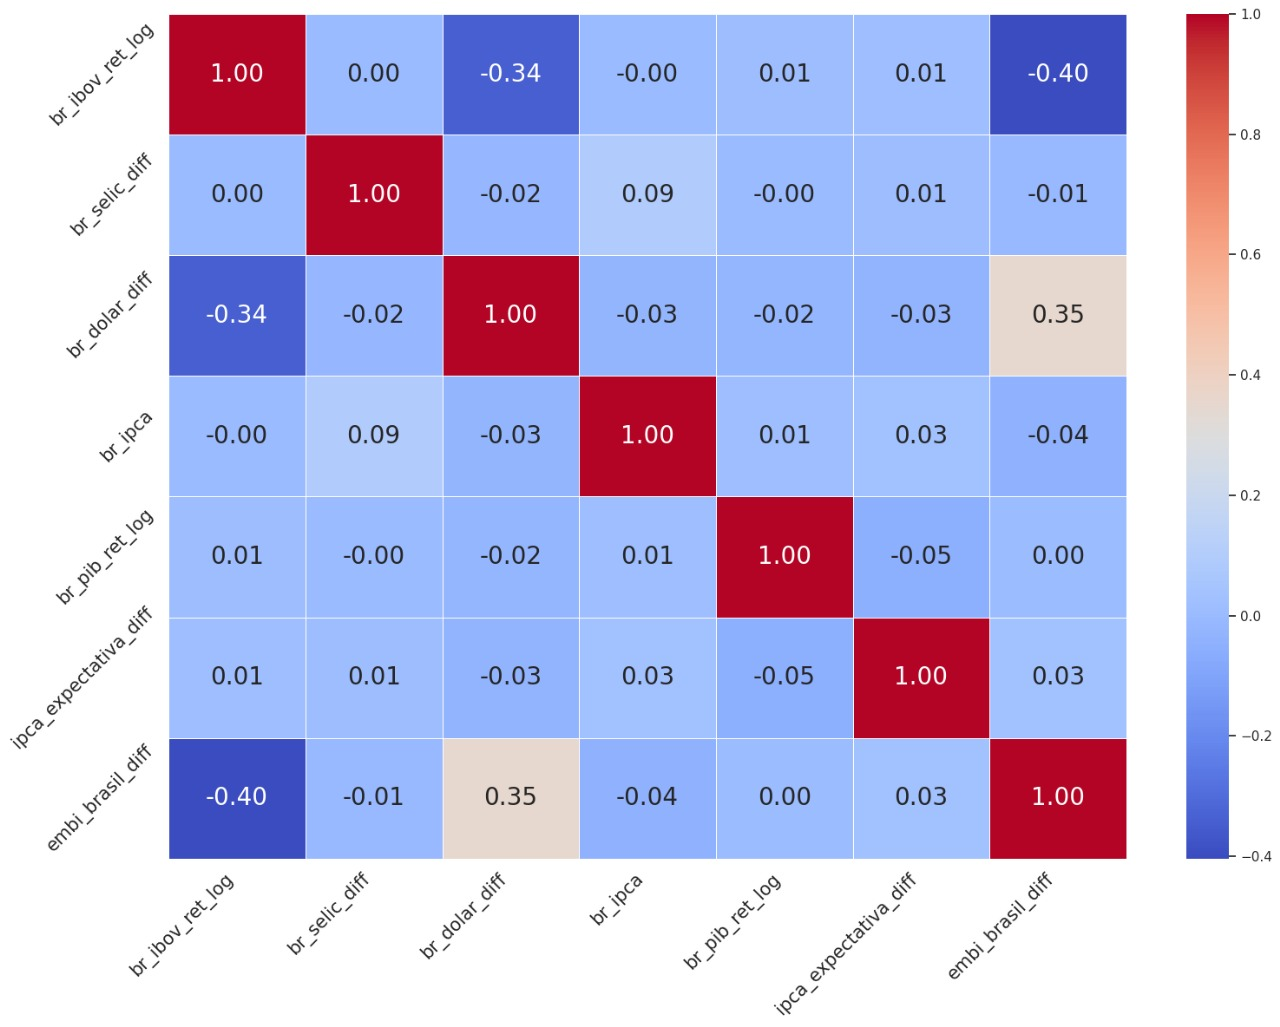
\includegraphics[scale=0.35]{mapa-de-calor-transformada-4.png}
	\end{center}
    \caption{\label{fig:mapa-calor}Mapa de Calor - Correlação das Variáveis Transformadas (Fonte: Autor)}
\end{figure}

A validade estatística dos modelos de séries temporais exige que as variáveis sejam estacionárias. Foram aplicados os testes ADF (Augmented Dickey-Fuller) e KPSS (Kwiatkowski-Phillips-Schmidt-Shin) tanto nas séries originais quanto nas transformadas. A maioria das séries em nível apresentou sinais claros de não estacionariedade (p-valor alto no ADF, baixo no KPSS). Após a transformação, todas as variáveis mostraram-se estacionárias, com p-valores do ADF próximos de zero e p-valores do KPSS acima de 0,05.

\begin{figure}[htb]
	
	\begin{center}
	    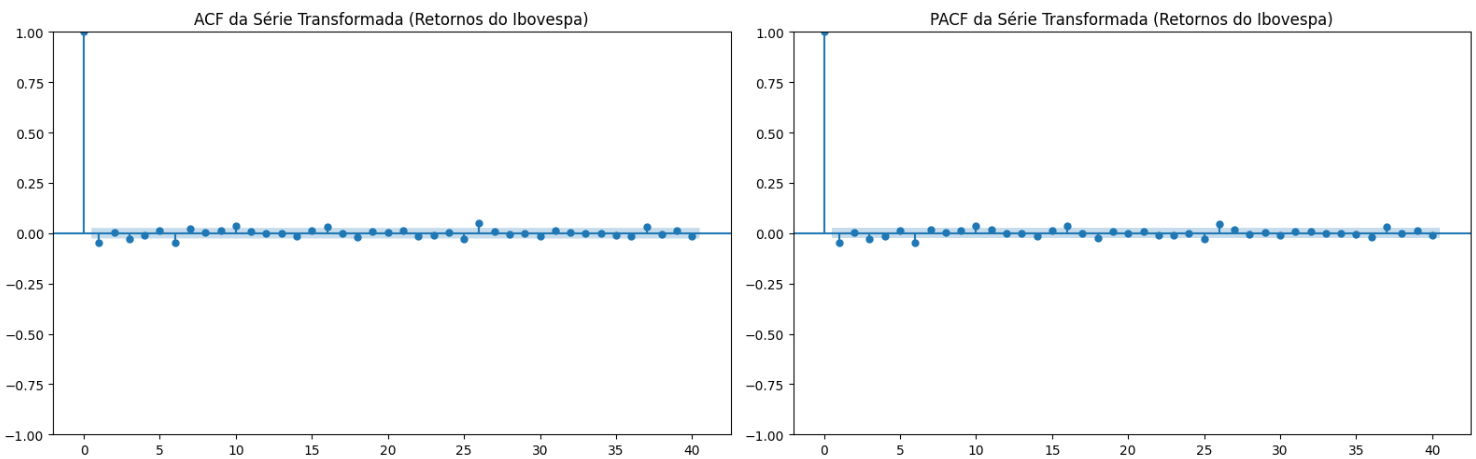
\includegraphics[scale=0.3]{acf-pacf.png}
	\end{center}
	\caption{\label{fig:acf-pacf}Gráficos ACF e PACF da série transformada (Fonte: Autor)}
\end{figure}

Esses resultados garantem a adequação dos dados para modelagens posteriores, evitando vieses nas inferências.

Um modelo ARIMA foi ajustado à série de retornos logarítmicos do Ibovespa. Com base na análise de ACF/PACF (Figura \ref{fig:acf-pacf}) e na seleção automática via critério AIC, foi identificado o modelo ARIMA(4, 0, 3). O teste de Ljung-Box apresentou p-valor de 0,29, indicando que não há autocorrelação significativa nos resíduos — o que sugere que o modelo conseguiu capturar adequadamente a dinâmica interna da série.

Este resultado estabelece um benchmark univariado, baseado apenas no comportamento passado do índice.

Em seguida, foi estimado um modelo de regressão linear múltipla com os retornos do Ibovespa como variável dependente e as variáveis transformadas como preditoras. Observou-se que \textbf{R² = 0{,}209}. Embora o valor seja considerado razoável em contextos de alta volatilidade como o mercado financeiro, ele também evidencia uma limitação importante do modelo MQO: sua baixa capacidade explicativa frente à complexidade das relações econômicas envolvidas. Além disso, o MQO assume linearidade, homocedasticidade e ausência de interações complexas entre variáveis — suposições muitas vezes violadas em séries financeiras. Essas restrições reforçam a necessidade de empregar modelos mais flexíveis e robustos, como GAM, BSTS e Causal Forest, que são capazes de capturar não linearidades, efeitos dinâmicos e relações causais heterogêneas com maior precisão e interpretabilidade. Identificação de dois preditores estatisticamente significativos: variação do dólar, com impacto negativo e variação do risco-país (EMBI+), também com impacto negativo. Os testes diagnósticos indicaram ausência de multicolinearidade (VIF baixo), como visto na Tabela \ref{tab:vif}, mas rejeição das hipóteses de normalidade e homocedasticidade dos resíduos.

Essas falhas nos pressupostos justificam o avanço para modelos mais sofisticados, como os Generalized Additive Models (GAM), que serão empregados na próxima fase.


\begin{table}[ht!]
\centering
\begin{tabular}{|l|c|}
\hline
\textbf{Variável} & \textbf{VIF} \\ \hline
Constante (intercepto do modelo) & 2{,}8216 \\ \hline
Variação da taxa Selic & 1{,}0091 \\ \hline
Variação de câmbio dólar (venda) & 1{,}1439 \\ \hline
Índice de Preços ao Consumidor Amplo (IPCA) & 1{,}0119 \\ \hline
Retorno logarítmico do PIB  & 1{,}0039 \\ \hline
Variação da expectativa de inflação (IPCA esperado) & 1{,}0076 \\ \hline
Variação do risco-país (EMBI+ Brasil) & 1{,}1441 \\ \hline
\end{tabular}
\caption{Fatores de Inflação da Variância (VIF) para as variáveis explicativas}\label{tab:vif}
\end{table}

Para técnicas de explicação, pode-se considerar a técnica SHAP, baseada na teoria dos valores de Shapley, originalmente desenvolvida na teoria dos jogos cooperativos. SHAP atribui a cada variável explicativa uma contribuição média para a previsão individual feita pelo modelo, de forma justa e consistente \cite{lundberg2018consistentfeatureattributiontree}.

No presente trabalho, os valores de SHAP poderão ser aplicados aos modelos GAM e Causal Forest para explicar quais variáveis macroeconômicas têm maior influência nos retornos do Ibovespa em diferentes contextos, em quais observações específicas (por exemplo, semanas de alta inflação ou forte depreciação cambial) a taxa Selic ou o risco-país exerceram maior impacto e, além disso, a variação da direção e magnitude do efeito da mesma variável entre diferentes janelas temporais ou regimes econômicos.

Gráficos de dispersão SHAP serão utilizados para visualizar a relação entre o valor de uma variável e sua contribuição individual para o retorno estimado, permitindo análises como: "o aumento do risco-país gera efeito negativo crescente até certo limite, e depois se estabiliza?"

Já os gráficos de dependência parcial (PDPs) serão aplicados principalmente ao modelo GAM, cuja estrutura aditiva permite uma decomposição natural dos efeitos marginais. PDPs mostram como a previsão média do modelo muda ao variar uma única variável explicativa, mantendo as demais constantes \cite{Friedman2001Machine}.

Esses gráficos são especialmente úteis para visualizar não linearidades (ex: efeito saturado ou em forma de U da inflação sobre os retornos), comparar efeitos marginais entre diferentes variáveis sob a mesma escala e validar se os efeitos estimados são economicamente coerentes (por exemplo, aumento da Selic reduz o retorno esperado, exceto em períodos de hiperinflação).

% ---
% Finaliza a parte no bookmark do PDF, para que se inicie o bookmark na raiz
% ---
\bookmarksetup{startatroot}% 
% ---
\chapter{Plano de Trabalho e Cronograma}

Nesta seção, são apresentados o plano de atividades referentes ao Trabalho de Conclusão de
Curso II (TCC II) e o cronograma da pesquisa (Tabela \ref{tabela:cronograma}).


\begin{table}[!h]

\begin{center}
\begin{tabular}{|l|c|c|c|c|c|c|}
\hline
{\bf Atividade} &     Mês 1 &     Mês 2 &     Mês 3 &     Mês 4 &     Mês 5 &     Mês 6 \\
\hline
atividade 1 &     x       &      x     &        &        &          & \\
\hline
atividade 2 &            &      x      &      x     &            &            &            \\
\hline
atividade 3 &            &            &      x      &     x     &       &          \\
\hline
atividade 4 &            &            &            &          &     x    &            \\
\hline
atividade 5 &    &     &           &     &     &     x     \\
\hline
\end{tabular}
\caption{Tabela de cronograma de atividades.} \label{tabela:cronograma}
\end{center}
\end{table}

\begin{itemize}
\item \textbf{atividade 1:} Nesta atividade, será implementado o modelo GAM, com o objetivo de capturar as relações não-lineares que o modelo MQO não foi capaz de representar. A análise se concentrará na interpretação dos efeitos marginais por meio de gráficos de dependência parcial (PDP) e na comparação do desempenho em termos de $R^2$ e critérios de informação (AIC/BIC) com o modelo linear.

\item \textbf{atividade 2:} Esta etapa visa estimar o modelo BSTS, com o intuito de decompor a série temporal dos retornos do Ibovespa em componentes estruturais (como tendência e regressão). Será utilizada a análise de inclusão de variáveis ao longo do tempo, permitindo avaliar a relevância dinâmica dos preditores e suas mudanças de impacto sob diferentes regimes de mercado.

\item \textbf{atividade 3:} Aqui, será aplicado o modelo Causal Forest, com foco na inferência causal heterogênea. Será definido um “tratamento” exógeno (como um choque no risco-país) para estimar seu efeito causal sobre os retornos do Ibovespa. A análise também identificará variações desse efeito condicional em diferentes contextos econômicos.

\item \textbf{atividade 4:} Na quarta atividade, será realizada uma análise comparativa entre todos os modelos utilizados ao longo do trabalho (ARIMA, MQO, GAM, BSTS e Causal Forest). Serão consolidadas métricas de desempenho preditivo e interpretabilidade. A técnica SHAP será aplicada sobre o modelo mais complexo para validar a importância das variáveis de forma transparente.

\item \textbf{atividade 5:} Esta última etapa será dedicada à consolidação da monografia. Incluirá a redação final dos capítulos de metodologia e resultados, a elaboração da conclusão geral do trabalho, a revisão integral do texto e a preparação da apresentação para a banca avaliadora.

\end{itemize}


% ---
% Conclusão
% ---
\chapter{Conclusão}

Os resultados obtidos até esta etapa confirmam a importância de um tratamento cuidadoso das séries temporais utilizadas no projeto, especialmente no que se refere à necessidade de transformações para garantir a estacionariedade e evitar regressões espúrias. A análise exploratória, os testes de estacionariedade e os primeiros modelos estimados,como ARIMA e regressão linear com MQO, serviram como linha de base para avaliar a previsibilidade e os fatores que explicam os retornos do Ibovespa a partir de variáveis macroeconômicas e financeiras.

Apesar de sua relevância teórica e interpretabilidade direta, os modelos econométricos tradicionais mostraram limitações importantes. O modelo ARIMA, por ser univariado, não incorpora variáveis explicativas externas e apenas projeta a série com base em sua própria dinâmica. Já o modelo MQO, embora tenha permitido identificar relações estatisticamente significativas (como os efeitos negativos do câmbio e do risco-país), apresentou baixa capacidade preditiva (R² = 0,209) e falhas nos pressupostos fundamentais, como homocedasticidade e normalidade dos resíduos. Além disso, ambos os modelos são incapazes de capturar não linearidades complexas, efeitos interativos e mudanças estruturais ao longo do tempo, características recorrentes em mercados financeiros.

Diante dessas limitações, torna-se evidente a necessidade de incorporar modelos mais flexíveis e robustos, capazes de capturar a complexidade do comportamento do mercado sem abrir mão da transparência interpretativa. A próxima fase do projeto se concentrará na aplicação de técnicas de inteligência artificial interpretável, que representam um avanço tanto do ponto de vista metodológico quanto prático:

O GAM (Generalized Additive Model) permite modelar relações não lineares entre variáveis de forma transparente, decompondo efeitos marginais com funções suavizadas. Isso possibilita, por exemplo, identificar comportamentos econômicos com pontos de inflexão ou efeitos saturados, o que não seria detectado por uma regressão linear. O BSTS (Bayesian Structural Time Series) oferecerá uma abordagem probabilística e temporalmente sensível, permitindo decompor a série em tendência, sazonalidade e regressão com covariáveis. Sua estrutura bayesiana facilita a inclusão de incertezas e o rastreamento da importância dinâmica dos preditores ao longo do tempo. O Causal Forest, por sua vez, será utilizado para investigar efeitos causais que variam entre diferentes contextos, possibilitando estimar como mudanças externas (como alterações súbitas na taxa de juros ou aumentos no risco-país) afetam o comportamento dos retornos do Ibovespa. A técnica permite identificar subgrupos com respostas diferenciadas, indo além das médias globais e revelando nuances causais mais sofisticadas.

Ao utilizar essas abordagens, o projeto buscará superar os limites da modelagem linear tradicional, entregando resultados que sejam não apenas estatisticamente robustos, mas também compreensíveis e acionáveis para analistas, investidores e formuladores de política econômica. Além disso, o uso de técnicas como SHAP e PDP contribuirá para validar e visualizar os efeitos estimados, reforçando o compromisso do trabalho com a explicabilidade e a transparência dos modelos.

Além da contribuição metodológica, este trabalho possui relevância científica específica para o campo de economias emergentes. O Brasil apresenta dinâmicas de risco, câmbio e resposta a choques externos que diferem estruturalmente de mercados desenvolvidos, tornando indispensável que os modelos aplicados sejam não apenas acurados, mas também interpretáveis o suficiente para que analistas e gestores possam identificar quando e por que um modelo falha nesse ambiente. A capacidade de auditar o comportamento do modelo diante de episódios como crises cambiais, choques políticos ou reversões abruptas de política monetária representa, em si, um resultado científico relevante — e é precisamente essa capacidade que a abordagem de inteligência artificial interpretável proposta neste trabalho busca entregar.

Conclui-se, portanto, que o uso de IA interpretável representa não apenas uma evolução técnica, mas também uma exigência prática e ética em ambientes financeiros complexos. O projeto avança agora para uma fase decisiva, em que a combinação entre flexibilidade preditiva e clareza interpretativa poderá revelar novos insights sobre os fatores macroeconômicos que moldam o comportamento do mercado brasileiro.

% ----------------------------------------------------------
% ELEMENTOS PÓS-TEXTUAIS
% ----------------------------------------------------------
\postextual


% ----------------------------------------------------------
% Referências bibliográficas
% ----------------------------------------------------------
%\bibliographystyle{plain}
\bibliography{references}

% ----------------------------------------------------------
% Glossário
% ----------------------------------------------------------
%
% Consulte o manual da classe abntex2 para orientações sobre o glossário.
%
%\glossary


% ---
\end{document}
